%
%  untitled
%
%  Created by Colin Williams on 2012-01-06.
%  Copyright (c) 2012 __MyCompanyName__. All rights reserved.
%
\documentclass[]{article}

% Use utf-8 encoding for foreign characters
\usepackage[utf8]{inputenc}

% Setup for fullpage use
\usepackage{fullpage}

% Uncomment some of the following if you use the features
%
% Running Headers and footers
%\usepackage{fancyhdr}

% Multipart figures
%\usepackage{subfigure}

% More symbols
%\usepackage{amsmath}
%\usepackage{amssymb}
%\usepackage{latexsym}

% Surround parts of graphics with box
\usepackage{boxedminipage}

% Package for including code in the document
\usepackage{listings}

% If you want to generate a toc for each chapter (use with book)
\usepackage{minitoc}

% This is now the recommended way for checking for PDFLaTeX:
\usepackage{ifpdf}
\usepackage{comment}

%\newif\ifpdf
%\ifx\pdfoutput\undefined
%\pdffalse % we are not running PDFLaTeX
%\else
%\pdfoutput=1 % we are running PDFLaTeX
%\pdftrue
%\fi


\usepackage{array}
\usepackage{url}
\usepackage{listings}
\usepackage{color}
\usepackage{amsmath}
\usepackage{mathtools}

\definecolor{dkgreen}{rgb}{0,0.6,0}
\definecolor{gray}{rgb}{0.5,0.5,0.5}
\definecolor{mauve}{rgb}{0.58,0,0.82}

\lstset{
  language=Java,
  tabsize=4,
  showstringspaces=false,
  basicstyle=\tt,
  numberstyle=\tiny\color{gray},      % line number style
  keywordstyle=\color{blue},          % keyword style
  commentstyle=\color{dkgreen},       % comment style
  stringstyle=\color{mauve},          % string literal style
}

\ifpdf
\usepackage[pdftex]{graphicx}
\else
\usepackage{graphicx}
\fi
\title{Negotiation User Guide}
\author{T. Baarslag, W. Pasman, K. Hindriks, D. Tykhonov, W. Visser, M. Hendrikx}

\date{\today}

% Alter some LaTeX defaults for better treatment of figures:
    % See p.105 of "TeX Unbound" for suggested values.
    % See pp. 199-200 of Lamport's "LaTeX" book for details.
    %   General parameters, for ALL pages:
    \renewcommand{\topfraction}{0.9}	% max fraction of floats at top
    \renewcommand{\bottomfraction}{0.8}	% max fraction of floats at bottom
    %   Parameters for TEXT pages (not float pages):
    \setcounter{topnumber}{2}
    \setcounter{bottomnumber}{2}
    \setcounter{totalnumber}{4}     % 2 may work better
    \setcounter{dbltopnumber}{2}    % for 2-column pages
    \renewcommand{\dbltopfraction}{0.9}	% fit big float above 2-col. text
    \renewcommand{\textfraction}{0.07}	% allow minimal text w. figs
    %   Parameters for FLOAT pages (not text pages):
    \renewcommand{\floatpagefraction}{0.7}	% require fuller float pages
	% N.B.: floatpagefraction MUST be less than topfraction !!
    \renewcommand{\dblfloatpagefraction}{0.7}	% require fuller float pages

	% remember to use [htp] or [htpb] for placement
	
\begin{document}

\ifpdf
\DeclareGraphicsExtensions{.pdf, .jpg, .tif}
\else
\DeclareGraphicsExtensions{.eps, .jpg}
\fi

\maketitle

\newcommand\Genius{{\sc Genius}}

\abstract{\noindent In \Genius, you can implement and analyze an agent that negotiates on your behalf. This document describes how you can install the required environment, work with the provided agents, and write, compile, and run such an agent yourself.}

\pagebreak
\tableofcontents

\pagebreak
\section{Theory Crash Course}
This section provides a crash course on some essential theory needed to understand the negotiation system. Furthermore, it provides an overview of the features of a negotiation implemented in \Genius.

\subsection{Negotiation Protocol}
The negotiation protocol determines the overall order of actions during a negotiation. Agents are obliged to stick to this protocol, as deviations from the protocol are caught and penalized. This section discusses the details of the bilateral alternating offers protocol used in \Genius.

In the bilateral alternating offers protocol two parties -- agent $A$ and agent $B$ -- take turns. Agent $A$ starts the negotiation. Each turn an agent presents one of the three possible actions:

\begin{center}
\begin{tabular}{cm{0.6\textwidth}}
\hline
\textsc{Accept} & This action indicates that agent accepts the opponent's last bid.\\
\hline
\textsc{Offer} & This action represents the bid made by an agent.\\
\hline
\textsc{EndNegotiation} & This action indicates that the agent terminates the negotiation.\\
\hline
\end{tabular}
\end{center}

When it is an agent's turn, it is informed about the opponent's action. Based on the opponent's action the agent comes up with a action, which it presents to the opponent. Sequentially, the opponent presents a counter action. This process goes on until the negotiation finishes in one of the following ways:
\begin{itemize}
	\item An agent accepts the opponent's offer using the action \textsc{Accept}. The utility of the opponent's last bid is determined for both agents according to their preference profiles. The opponent is informed of acceptance via the \textit{ReceiveMessage} method.
	\item The action returned by an agent is \textsc{EndNegotiation}. In this case the score of both agents is set to their reservation value.
	\item Finally, if an agent does not follow the protocol -- for instance by sending an action that is not one of the above or by crashing -- the agent's utility is set to reservation value, whereas the opponent is awarded the utility of the last offer.
\end{itemize}
 
\subsection{Reservation Value}
A reservation value is a real-valued constant that sets a threshold below which a rational agent should not accept any offers. Intuitively, a reservation value is the utility associated with the Best Alternative to a Negotiated Agreement (BATNA).

A reservation value is the utility that an agent will obtain if no agreement is realized in a negotiation session. This can happen either if an agent leaves the negotiation, or by not reaching an agreement before the deadline. In other words: either the negotiating parties agree on an outcome $\omega$, and both agents receive the associated utility of $\omega$, or no agreement is reached, in which case both agents receive their reservation value instead. Reservation values typically differ for each negotiation agent. In case no reservation value is set in a profile, it is assumed 0.


\subsection{Time Pressure}
A negotiation lasts a predefined time in seconds, or alternatively rounds. In \Genius~the time line is \emph{normalized}, i.e.: time $t \in [0, 1]$, where $t = 0$ represents the start of the negotiation and $t = 1$ represents the deadline. Notice that manipulation of the remaining time can be a factor influencing the outcome.

There is an important difference between a time-based and rounds-based protocol. In a time-based protocol the computational cost of an agent should be taken into account as it directly influences the amount of bids which can be made. In contrast, for a rounds-based negotiation the time can be thought of as frozen inside a round; therefore computational cost does not play a role.

Apart from a deadline, a scenario may also feature \emph{discount factors}. Discount factors decrease the utility of the bids under negotiation as time passes. While time is shared between both agents, the discount generally differs per agent. The implementation of discount factors is as follows: let $d$ in $[0, 1]$ be the discount factor that is specified in the preference profile of an agent; let $t$ in $[0, 1]$ be the current normalized time, as defined by the timeline; we compute the discounted utility $U_D^t$ of an outcome $\omega$ from the undiscounted utility function $U$ as follows:
\begin{eqnarray}
U_D^t(\omega) = U(\omega) \cdot d^t
\end{eqnarray}
If $d = 1$, the utility is not affected by time, and such a scenario is considered to be undiscounted, while if $d$ is very small there is high pressure on the agents to reach an agreement. Note that discount factors are part of the preference profiles and therefore different agents may have a different discount factor.

If a discount factor is present, reservation values will be discounted in exactly the same way as the utility of any other outcome. It is worth noting that, by having a discounted reserve price, it may be rational for an agent to end the negotiation early and thereby default to the reservation value.

\subsection{Negotiation Objects}
Agent participating in a negotiation interact in a scenario. A scenario specifies the possible bids by using the domain and the preferences for each agent with a utility space for each agent. Figure~\ref{Fig:overviewStructures} provides an overview of the relation between the domain and the utility space of an agent.

\begin{figure}[htb]
	\centering
	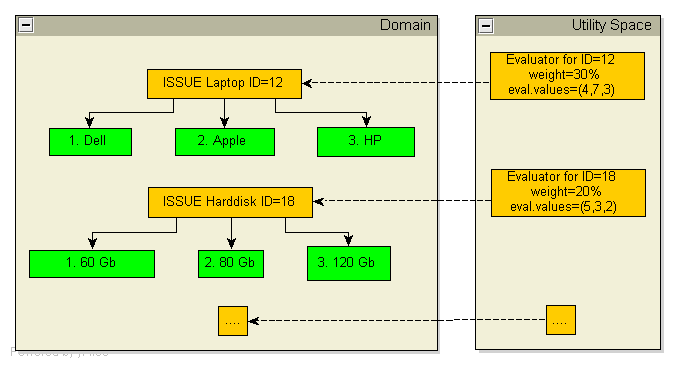
\includegraphics[width=0.5\textwidth]{media/datastructures.png}
	\caption{Overview of the data structures and relations.}\label{Fig:overviewStructures}
\end{figure}

The \textit{Domain} describes which issues are the subject of the negotiation and which values an issue can attain. To give a concrete example of a domain: in the laptop domain the issues are ``laptop'', ``harddisk'' and ``monitor''. In the laptop domain the issues can only attain discrete values, e.g. the ``harddisk'' issue can only have the values ``60 Gb'', ``80 Gb'' and ``120 Gb''. These issues are all instance of \textit{IssueDiscrete}.

Combining these concepts, an agent can formulate a \textit{Bid}: a mapping from each issue to a value. A valid bid in the laptop domain is for example a Dell laptop with 80 Gb and a 17' inch monitor.

The \textit{UtilitySpace} specifies the preferences of the bids for an agent. Using a utility space the utility of a bid can be calculated using the evaluator of each issue. The evaluator of an issue maps the evaluation of a value-- which is specified in the preference profile -- to a utility for that issue. The evaluator also specifies the importance of the issue relative to the other issues in the form of a weight. The weights of all issues sum up to 1.0. To illustrate, the ``harddisk'' issue is of the type \textit{IssueDiscrete}, and therefore its evaluator is of the type \textit{EvaluatorDiscrete}.

In general, given the set of all bids, there are a small subset of bids which are more preferred as outcomes by both agents. Identifying these special bids may lead to a better agreement for both parties. We discuss the optimality of a bid in the next section.

\subsection{Optimality of a Bid}
Before discussing the optimality of a bid, we first need to formalize the concept of a bid. A bid is a set of chosen values $v_1, \ldots, v_n$  for each of the $N$ issues. Each of these values has been assigned an evaluation value $\text{eval}(v_i)$ in the utility space. The utility is the weighted sum of the normalized evaluation values.

\begin{equation}
	U(v_1, \ldots, v_n) = \sum_{i=1}^{N} w_i \dfrac{\text{eval}(v_i)}{\text{max}(\text{eval}(v_i))}
	\label{eqn:Utility}
\end{equation}

For a single agent, the optimal bid is of maximum utility for the agent. Often this bid has a low utility for the opponent, and therefore the chance of agreement is low. A more general notion of optimality of a negotiation involves the utility of both agents.
\begin{figure}[htb]
	\centering
	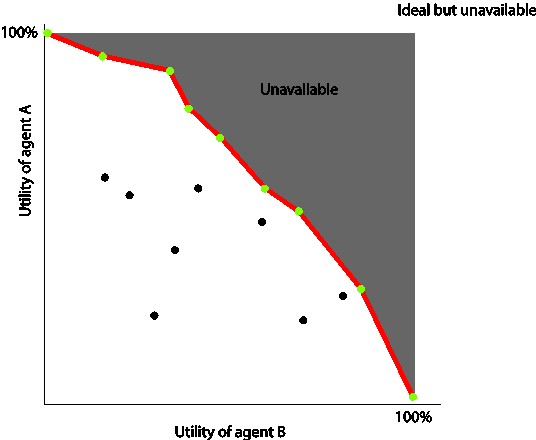
\includegraphics[width=0.37\textwidth]{media/image5.png}
\caption{A point indicates the utility for both agents of a bid. The red line is the Pareto optimal frontier.}\label{Fig:utility plot}
\end{figure}

There are multiple ways to define a more global ``optimum''. One approach to optimality is that a bid is not optimal for both parties if there is another bid that has the higher utility for one party, and at least equal utility for the other party. Thus, only bids in Figure~\ref{Fig:utility plot} for which there is no other bid at the top right is optimal. This type of optimality is called Pareto optimality and forms an important concept in automated negotiation. The collection of Pareto optimal bids is called the Pareto optimal frontier.

A major challenge in a negotiation using the bilateral alternating offers protocol is that agents hide their preference profile. This entails that an agent does not know which bid the opponent prefers given a set of bids. This problem can be partly resolved by building a model of the opponent's preferences by analyzing the negotiation trace. Each turn the agent can now offer the best bid for the opponent given a set of similar preferred bids for itself. By default, there are already a few opponent models implemented in \Genius, such as the \textit{HardHeadedFrequencyModel} used by the \textit{HardHeaded} agent which won the ANAC2011.
 
\section{Running the Environment}
The negotiation environment has been tested extensively on Microsoft Windows. It should run on any machine running Java 6 or higher, including Solaris and Linux distributions. There are known issues with Linux (in particular Ubuntu and SUSE) mainly involving the visualization of the GUI. Please report any bugs found to \url{ai@mmi.tudelft.nl}.

To install the environment, the file \texttt{negotiator.zip} can be downloaded. Unzip the file at a convenient location on your machine. This will result in a package containing the following files:

\begin{itemize}
	\item \texttt{userguide.pdf}, this document;
	\item \texttt{negosimulator.jar}, the negotiation simulator;
	\item a \texttt{templates} folder, containing various scenarios.
\end{itemize}

When you run the negosimulator (by double-clicking the application or using open with and then selecting Java), progress messages and error messages are printed mainly to the standard output. On Mac OSX you can view these messages by opening the console window (double-click on Systemdisk/Applications/Utilities/Console.app). On Windows this is not directly possible. Console output can be read only if you start the application from the console window by hand, as follows. Go to the directory with the negosimulator and enter
\texttt{java -jar negosimulator.jar}.
This will start the simulator, and all messages will appear in the console window. You may see some errors and warnings that are non-critical.

\section{Scenario Creation}
A negotiation can be modeled in \Genius~by creating a scenario. A scenario consists of a domain specifying the possible bids and a set of preference profiles corresponding to the preferences of the bids in the domain. This section discusses how to create a domain and a preference profile.

\subsection{Basic GUI Components}
Start \Genius~by following the instructions in the previous section. After starting the simulator a screen similar to Figure~\ref{Fig:negosimulator start} is shown. This screen is divided in three portions:

\begin{itemize}
	\item The \textbf{Menubar} allows us to start a new negotiation.
	\item The \textbf{Components Window} shows all available scenarios and agents.
	\item The \textbf{Status Window} shows the negotiation status or selected domain/preference profile.
\end{itemize}

\begin{figure}[htb]
	\centering
	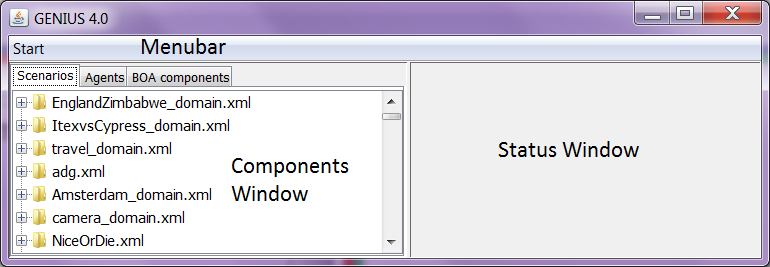
\includegraphics[width=0.6\textwidth]{media/image6.png}
\caption{The negosimulator right after start-up.}\label{Fig:negosimulator start}
\end{figure}

\subsection{Creating a Domain}
By right clicking on the list of available scenarios in the Components Window a popup menu with the option to create a new domain is shown. After clicking this option it is requested where the domain should be saved. As a domain is accompanied by a set of preference profiles, it is recommended to save the file in a new directory in the templates folder. After saving the domain a window similar to Figure~\ref{Fig:newdomain} is shown. Initially, a domain contains zero issues. We can simply add an issue by pressing the ``Add issue'' button. This results in the opening of a dialog similar to Figure~\ref{fig:createIssueD}.

\begin{figure}[htb]
	\centering
	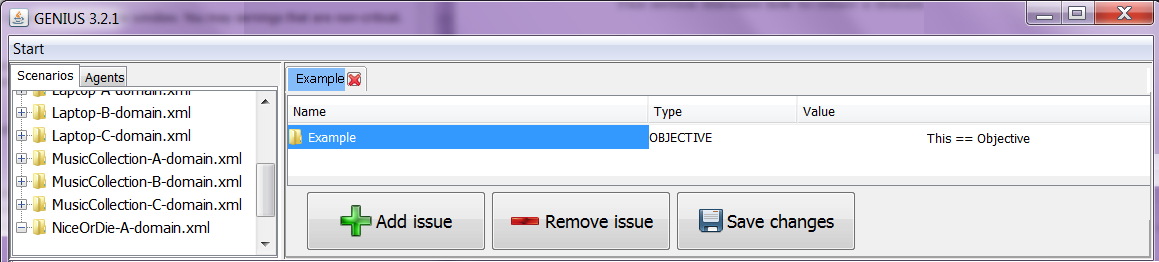
\includegraphics[width=0.7\textwidth]{media/image7.png}
\caption{The negosimulator after loading the laptop domain.}\label{Fig:newdomain}
\end{figure}

The current version of \Genius~supports the creation of discrete and integer issues. Starting with a discrete issue, the values of the issue should be specified. In Figure~\ref{fig:createIssueD} we show the values of the issue ``Harddisk''. Note the empty evaluation values window, later on when creating a preference profile we will use this tab to specify the preference of each value.

Instead of a discrete issue, we can also add an integer issue as shown in Figure~\ref{fig:createIssueI}. For an integer issue we first need to specify the lowest possible value and the highest value, for example the price you want to pay for a second hand car may be in the range $[700, 900]$. Next, when creating a preference profile we need to specify the utility of the lowest possible value (700) and the highest value (900). During the negotiation we can offer any value for the issue within the specified range.

The next step is to press ``Ok'' to add the issue. Generally, a domain consists of multiple issues. We can simply add the other issues by repeating the process above. If you are satisfied with the domain, you can save it by pressing  ``Save changes''.

Finally, note that the issues of a domain can only be edited if the scenario does not (yet) specify preference profiles. This is to avoid inconsistencies between the preference profiles and the domains. 

\begin{figure}[ht]
\begin{minipage}[b]{0.45\linewidth}
\centering
	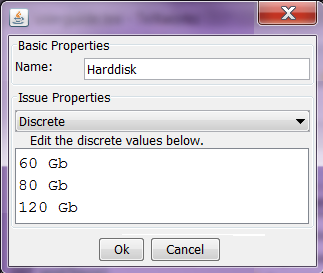
\includegraphics[width=0.8\textwidth]{media/image7a.png}
\caption{Creating a discrete issue.}
\label{fig:createIssueD}
\end{minipage}
\begin{minipage}[b]{0.45\linewidth}
\centering
	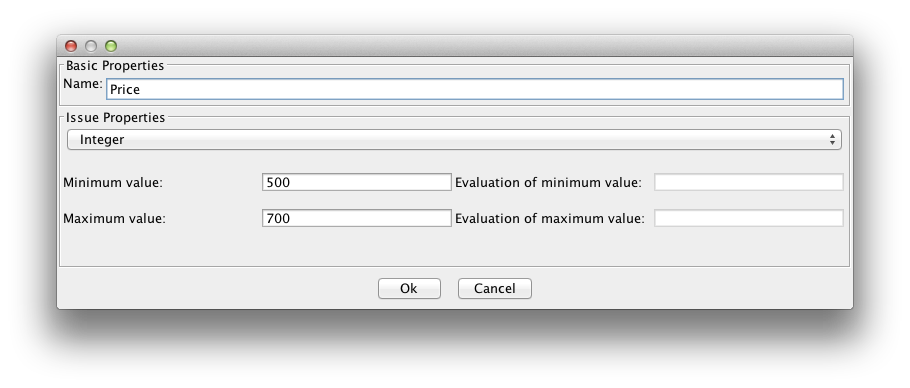
\includegraphics[width=0.8\textwidth]{media/image7b.png}
\caption{Creating an integer issue.}\label{fig:createIssueI}
\end{minipage}
\end{figure}

\subsection{Creating a Preference Profile}
Now that we created a domain, the next step is to add a set of preference profiles. By right clicking on the domain a popup menu is opened which has an option to create a new preference profile. Selecting this option results in the opening of a new window which looks similar to Figure~\ref{fig:utilcreated}.

\begin{figure}[htb]
	\centering
	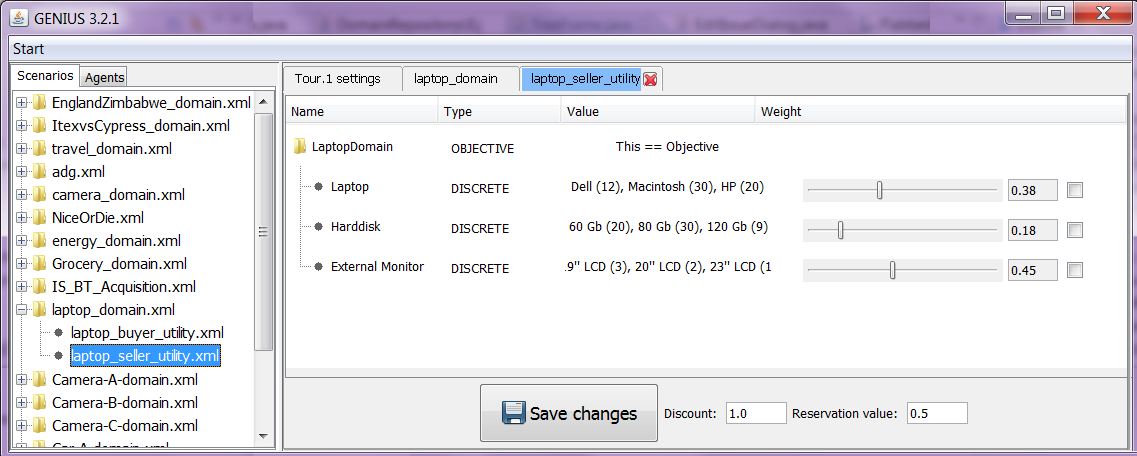
\includegraphics[width=0.8\textwidth]{media/image8.png}
\caption{The negosimulator after creating a new utility space.}\label{fig:utilcreated}
\end{figure}

Now you are ready to start customizing the preference profile. There are three steps: setting the importance of the issues, determining the preference of the values of the issues, and configuring the reservation value and discount. To start with the first step, you can adjust the relative weights of the issues by using the sliders next to that issue. Note that when you move a slider, the weights of the other sliders are automatically updated such that the all weights still sum up to one. If you do not want that the weight of another issue automatically changes, you can lock its weight by selecting the checkbox behind it. Now that we set the weights of the issues, it is a good idea to save the utility space.

The next and final step is to set the evaluation of the issues. To specify the evaluation of an issue you can double click it to open a new window looking similar to Figure~\ref{fig:createIssueD} or Figure~\ref{fig:createIssueI} depending on the type of the issue.

For a discrete issue we need to specify the evaluation value of each discrete value. A specific value can be assigned any positive non-zero integer as evaluation value. During the negotiation the utility of value is determined by dividing the value by the highest value for that particular issue. To illustrate, if we give 60 Gb evaluation 5, 80 Gb evaluation 8, and 120 Gb evaluation 10; then the utilities of these values are respectively 0.5, 0.8, and 1.0.

Specifying the preference of a integer issue is even easier. In this case we simply need to specify the utility of the lowest possible value and the highest possible value. The utility of a value in this range is calculated during the negotiation by using linear interpolation of the utilities of both given utilities.

The final step is to set the reservation value and discount of a preference profile. If you are satisfied with the profile you can save it by pressing ``Save changes''. 

\section{Running Negotiations}
This section discusses how to run a negotiation. There are three main modes to run a negotiation:

\begin{itemize}
	\item \textbf{Negotiation session}. A negotiation session concerns a single negotiation in which two agents compete. This mode is mainly intended for new users.
	\item \textbf{Tournament}. A tournament is a collection of sessions. Two sets of agents compete against each other on a set of domains. The results of the matches are stored in the ``log'' directory. These results can be more easily viewed by importing them into Excel and using pivot tables.
	\item \textbf{Distributed tournament}. A distributed tournament is a tournament which is stored in a database and can therefore be divided among multiple computers to speed up calculation.
\end{itemize}

Before going into detail on how each of these modes work, we first discuss the two types of agents which can be used: automated agents and non-automated agents. Automated agents are agents which can compete against other agents in a negotiation without relying on input by a user. In general, these agents are able to make a large amount of bids in a limited amount of time.

In contrast, non-automated agents are agents that are fully controlled by the user. These types of agents ask the user each round which action they should make. \Genius~by default includes the UIAgent -- which has a simple user interface -- and the more extensive Extended UIAgent.


\subsection{Running a Negotiation Session}
To run a negotiation session select ``Start'' and then ``Negotiation Session''. This opens a window similar to Figure~\ref{Fig:session}. The following parameters need to be specified to run a negotiation:
\begin{itemize}
	\item \textbf{Negotiation protocol}. The set of available protocols. Normally ``Alternating Offers'' is used.
	\item \textbf{Side A/Side B}. The configuration of both agents which negotiate against each other.
	\item \textbf{Preference profile}. The preference profile to be used by the agent of that side.
	\item \textbf{Agent name}. The agent which should participate in the negotiation.
\end{itemize}

\begin{figure}[htb]
	\centering
	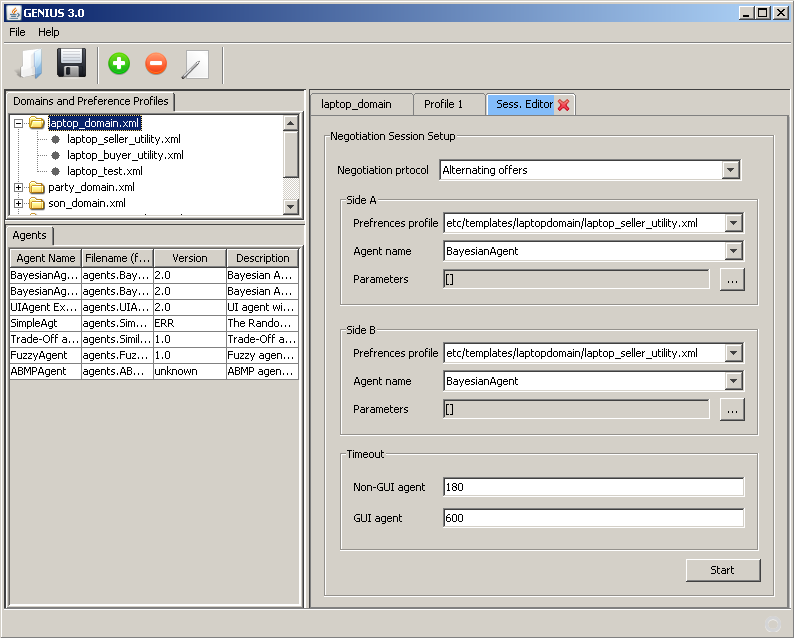
\includegraphics[width=0.6\textwidth]{media/image11.png}
\caption{A negotiation session.}\label{Fig:session}
\end{figure}


\subsection{Running a Tournament}
Besides running a single negotiation session, it is also possible to run a tournament. A tournament can be seen as a collection of sessions. In contrast to running a single session, the results of a tournament are stored in the ``log'' directory. These results can be easily analyzed by importing them into Excel an using pivot tables. A tournament can be created by first selecting ``Start'' and then ``Tournament''. The Tournament tab will appear similar to Figure~\ref{Fig:tournament}. This window shows a set of options which we need to specify. The value of an option can be specified by double clicking the option in the ``Values'' column.


\begin{figure}[htb]
	\centering
	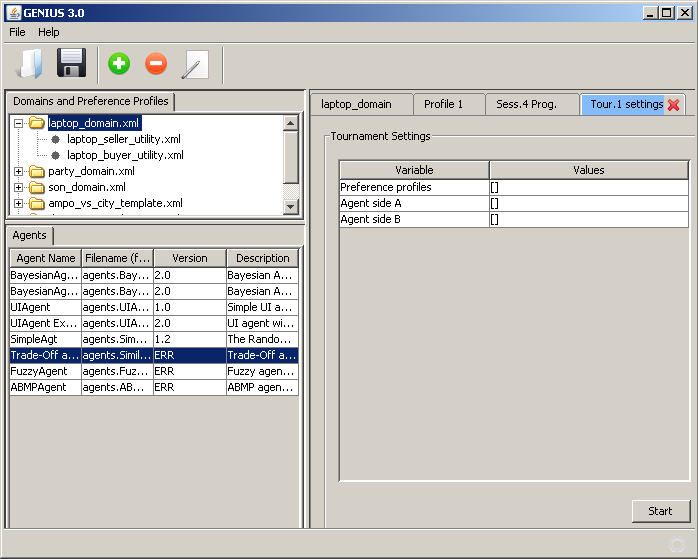
\includegraphics[width=0.8\textwidth]{media/image16.png}
\caption{Tournament tab.}\label{Fig:tournament}
\end{figure}

\begin{itemize}
	\item \textbf{Protocol}. The set of available protocols. Normally ``Alternating Offers'' is used.
	\item \textbf{Preference profiles}. The set of scenarios on which the agents should compete. Each selected scenario should feature at least two preference profiles.
	\item \textbf{Agent side A/B}. The set of agents in set A competes against all agents in set B.
	\item \textbf{Number of sessions}. The number of times each match should be repeated.
	\item \textbf{Tournament options}. Options which specify how to run the tournament (see below).
	\item \textbf{BOA Agent side A/B}. Type of agents which consist of multiple components (see~Section~\ref{sec:boa}).
\end{itemize}

In contrast to the negotiation session mode, a large set of tournament options can be specified which influence the composition and running of the tournament. There are four categories of options:
\begin{itemize}
	\item \textsc{Protocol settings}
	\begin{itemize}
		\item \textbf{Protocol mode}. Specifies if the negotiation features rounds or time. In a time-based negotiation there is an amount of time to reach an agreement. Time passes while an agent deliberates an action. In contrast, in a rounds-based negotiation the deadline is specified in rounds. An agent can take more time to compute an action as time does not pass within a round.
		\item \textbf{Deadline}. Depending on the protocol mode, this is the maximum amount of time in seconds or amount of rounds. Note that a single round corresponds to the turn of a single agent.
	\end{itemize}
	\item \textsc{Session generation}
	\begin{itemize}
		\item \textbf{Play both sides}. When generating the matches, should each pair of agents play both sides on a scenario or not.
		\item \textbf{Play against self}. An agent may be included both in the set Agent side A and side B. If this option is enabled an agent is allowed to play against itself. If disabled, the matches in which agents negotiate against themselves are removed.
	\end{itemize}
	\item \textsc{Logging}
	\begin{itemize}
		\item \textbf{Log detailed analysis}. Enabling this option activates a set of quality measures to capture the quality of the negotiation process. The quality measures are added to the default log. In addition, for the whole tournament an overview log is created. This log is prefixed with ``TM-''.
	\end{itemize}
	\item \textsc{Visualization}
	\begin{itemize}
		\item \textbf{Show all bids}. When enabled all bids in a scenario are visualized as red points in the negotiation status window. This option has a minor impact on performance.
		\item \textbf{Show last bid}. When enabled the last bid is marked with a special symbol to make it clear which move an agent performed. This has a negligible impact on performance.
		\item \textbf{Disable GUI}. When enabled most GUI elements are disabled. This speeds-up the negotiation up to a factor of 200 times. The progress of the tournament is printed to the console.
	\end{itemize}
\end{itemize}

\subsection{Running a Distributed Tournament}
A tournament quickly becomes practically too large to run. Running a distributed tournament resolves this problem as the tournament is stored in a database. Following, instances of \Genius~-- perhaps running on the same computer -- can connect to the database and process part of the tournament.

Before we can run a distributed tournament, we first need to setup a simple MySQL server which can be accessed by the computers. The installation of the database should include the ``InnoDB'' database engine. We will use this engine because it allows us to more easily remove old tournament data which we no longer need. Furthermore we recommend at least 50 Mb of free space. The required database structure can be created by using the SQL dump which can be found in the directory \textit{database}.

The next step is to specify a tournament to run. Towards this end, select ``Start'' and then ``Distributed tournament''. This opens a GUI similar to Figure~\ref{Fig:tournament}, except for the following four options:

\begin{itemize}
	\item \textbf{Database address}. The address of the database, for example \url{sql.ewi.tudelft.nl:3306/DG}.
	\item \textbf{Database user}. The username of the account for the database.
	\item \textbf{Database password}. The password of the user account for the database.
	\item \textbf{Database sessionname}. The identifier of the tournament. The identifier is needed as multiple distributed tournaments can be run at the same time.
\end{itemize}

After specifying the tournament and database parameters we can start the distributed tournament by pressing ``Start distributed tournament''. Selecting this button splits the tournament into smaller jobs which are stored in the database. The tournament is automatically started similar to a normal tournament. Now other computers can easily connect by specifying the database parameters and protocol and selecting ``Join distributed tournament''. Finally, after running the full tournament the results are sent to all computers and stored in the ``log'' directory. Figure~\ref{fig:dtournament} summarizes the process.

\begin{figure}[htb]
	\centering
	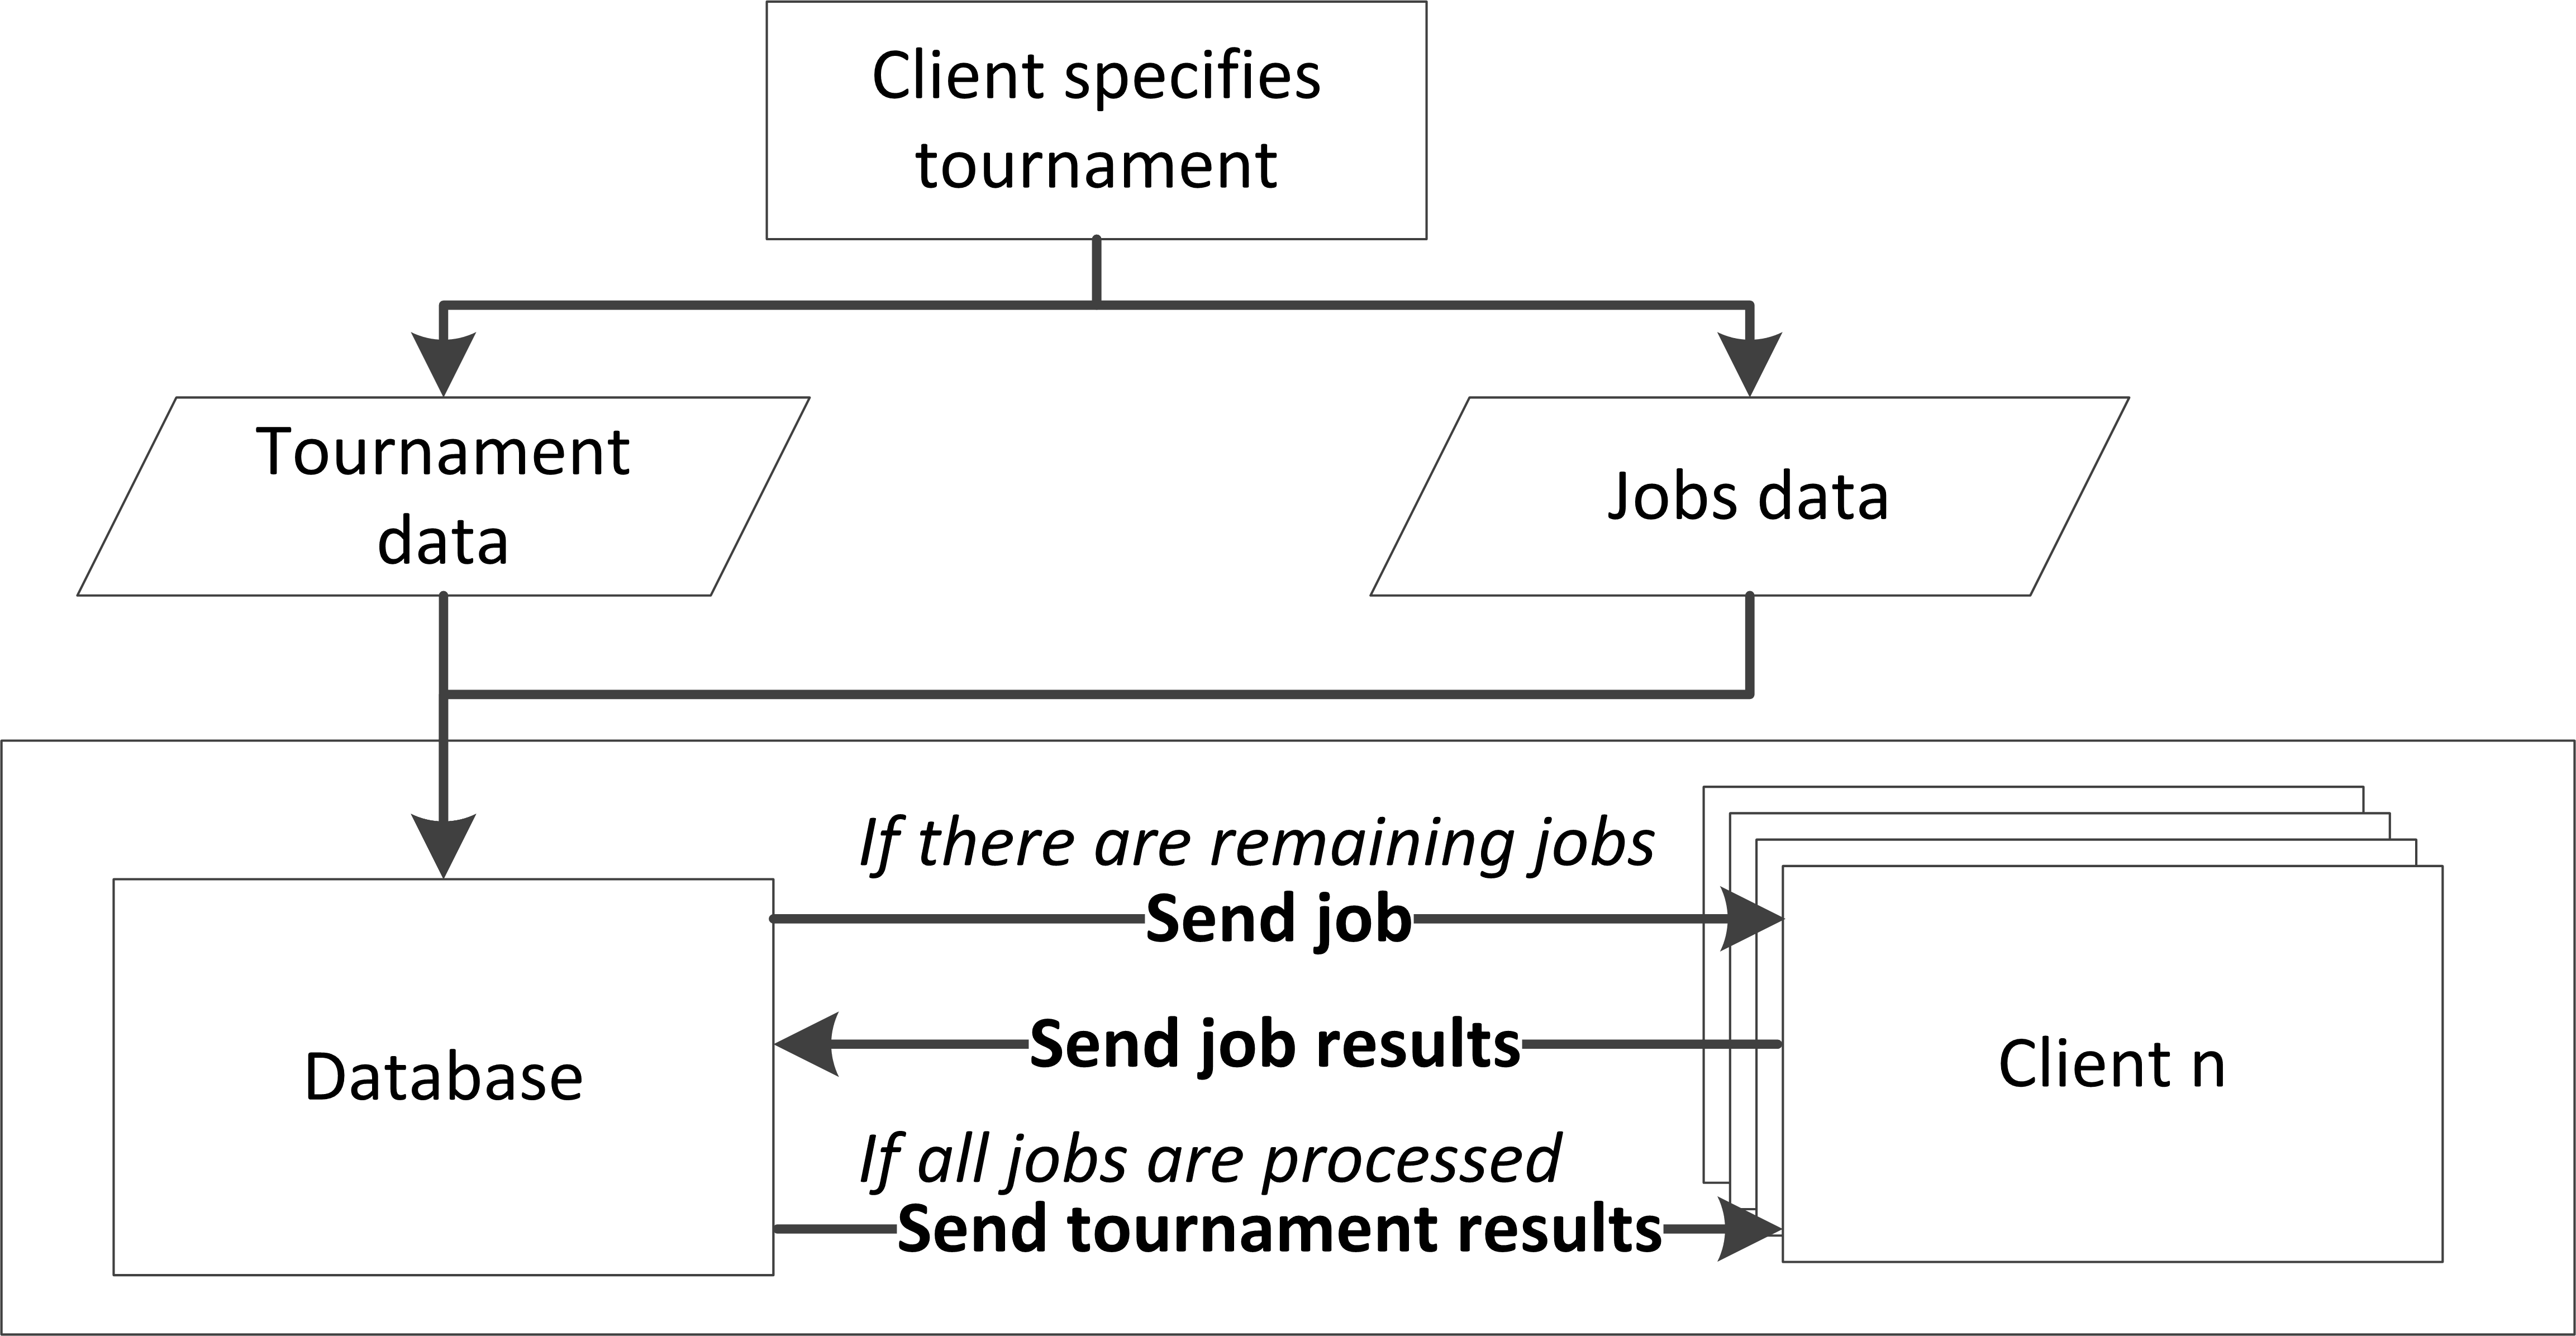
\includegraphics[width=0.50\textwidth]{media/DistributedGenius.png}
\caption{Distributed tournament process.}\label{fig:dtournament}
\end{figure}

It should be noted that currently there is no option in \Genius~to delete old tournament data. Therefore we recommend to install \textit{phpMyAdmin}. Using phpMyAdmin the old data of a tournament can be easily deleted by removing the tournament in the jobs table.

\section{Creating a Negotiation Agent}
This section discusses how to create a basic negotiation agent. A standard negotiation agent implements an agent as a single block of logic: a mix of a bidding strategy, acceptance strategy, and possibly an opponent model. In contrast, we recommend to split these components which can be done by implementing a BOA agent as discussed in Section~\ref{sec:boa}. The main advantage of a BOA agent is that existing components can be reused, allowing for easier agent development.

In this section we assume that you are familiar with programming in Java. In case you are not familiar with Java, please use the following link: \url{http://docs.oracle.com/javase/tutorial/index.html}. The Java API definitions can be found on \url{http://docs.oracle.com/javase/7/docs/api/index.html}.

The recommended way to create an agent is to create a new project in for example Eclipse or Netbeans. Next, add the \textit{negotiationsimulator.jar} as an external library to the project such that classes in the project can use the classes of \Genius. Finally, to create an agent create a new class and extend the \textit{negotiator.Agent} class. Table~\ref{tab:agentclass} shows the most important fields and methods of this class. For more information, please refer to the javadoc of \Genius. To implement your agent, you have to override the three methods: \textit{ReceiveMessage}, \textit{init}, and \textit{chooseAction}. An agent may consist of multiple classes.

\begin{table}
\begin{tabular}{m{0.9\textwidth}}
\hline
\texttt{UtilitySpace utilitySpace}\\
The preference profile of the scenario.\\
\hline
\texttt{Timeline timeline}\\
Use timeline for every time-related by using \texttt{getTime()}.\\
\hline
\texttt{double getUtility(Bid bid)}\\
A convenience method to get the utility of a bid taking the discount factor into account.\\
\hline
\texttt{void init()}\\
Informs the agent about beginning of a new negotiation session.\\
\hline
\texttt{void ReceiveMessage(Action opponentAction)}\\
Informs the agent which action the opponent did.\\
\hline
\texttt{Action chooseAction()}\\
This function should return the action your agent wants to make next.\\
\hline
\texttt{String getName()}\\
Returns the name of the agent. Please override this to give a proper name to your agent.\\
\hline
\end{tabular}
\caption{The most important methods and fields of the Agent class.}
\label{tab:agentclass}
\end{table}

\subsection{Receiving the Opponent's Action}
The \texttt{ReceiveMessage(Action opponentAction)} informs you that the opponent just did \texttt{opponentAction}. The \texttt{opponentAction} may be  \texttt{null} if you are the first to place a bid, or an \texttt{Offer}, \texttt{Accept} or \texttt{EndNegotiation} action.
The \texttt{chooseAction()} asks you to return an \texttt{Action} to make the next step in the negotiation.

In the SimpleAgent code, the following code is available for \texttt{ReceiveMessage}. The SimpleAgent stores the opponent's action to use it when choosing an action.

\begin{lstlisting}
public void ReceiveMessage(Action opponentAction) {
	actionOfPartner = opponentAction;
}
\end{lstlisting}

\subsection{Choosing an Action}
Below show the code of the method \texttt{chooseAction} for SimpleAgent. For safety, all code was wrapped in a try-catch block, because if our code would accidentally contain a bug we still want to return a good action (failure to do so is a protocol error and results in a utility of 0.0).

The sample code works as follows. If we are the first to place a bid, we place a random bid with sufficient utility (see the .java file for the details on that). Else, we determine the probability to accept the bid, depending on the utility of the offered bid and the remaining time. Finally, we randomly accept or pose a new random bid.

While this strategy works, in general it will lead to suboptimal results as it does not take the opponent into account. More advanced agents try to model the opponent's strategy or preference profile.

\begin{lstlisting}
public Action chooseAction() {
	Action action = null;
	try { 
		if (actionOfPartner == null) {
			action = chooseRandomBidAction();
		}
		if (actionOfPartner instanceof Offer) {
			Bid partnerBid = ((Offer) actionOfPartner).getBid();
			double offeredUtilFromOpponent = getUtility(partnerBid);
			// get current time
			double time = timeline.getTime();
			action = chooseRandomBidAction();
			
			Bid myBid = ((Offer) action).getBid();
			double myOfferedUtil = getUtility(myBid);
			
			// accept under certain circumstances
			if (isAcceptable(offeredUtilFromOpponent,myOfferedUtil,time)) {
				action = new Accept(getAgentID());
			}
		}
	} catch (Exception e) { 
		e.printStackTrace();
		action = new Accept(getAgentID()); // best guess if things go wrong. 
	}
	return action;
}
\end{lstlisting}

The method \textit{isAcceptable} implements the probabilistic acceptance function$P_\text{accept}$:

\begin{equation}
	P_\text{accept} = \dfrac{u - 2ut + 2\left(t - 1 + \sqrt{(t - 1)^2 + u(2t - 1)}\right)}{2t - 1}
\end{equation}
where $u$ is the utility of the bid made by the opponent (as measured in our utility space), and $t$ is the current time as a fraction of the total available time. Figure~\ref{Fig:Paccept} shows how this function behaves depending on the utility and remaining time. Note that this function only decides if a bid is acceptable or not. More advanced acceptance strategies also use the \texttt{EndNegotiation} action.
\begin{figure}[htb]
	\centering
	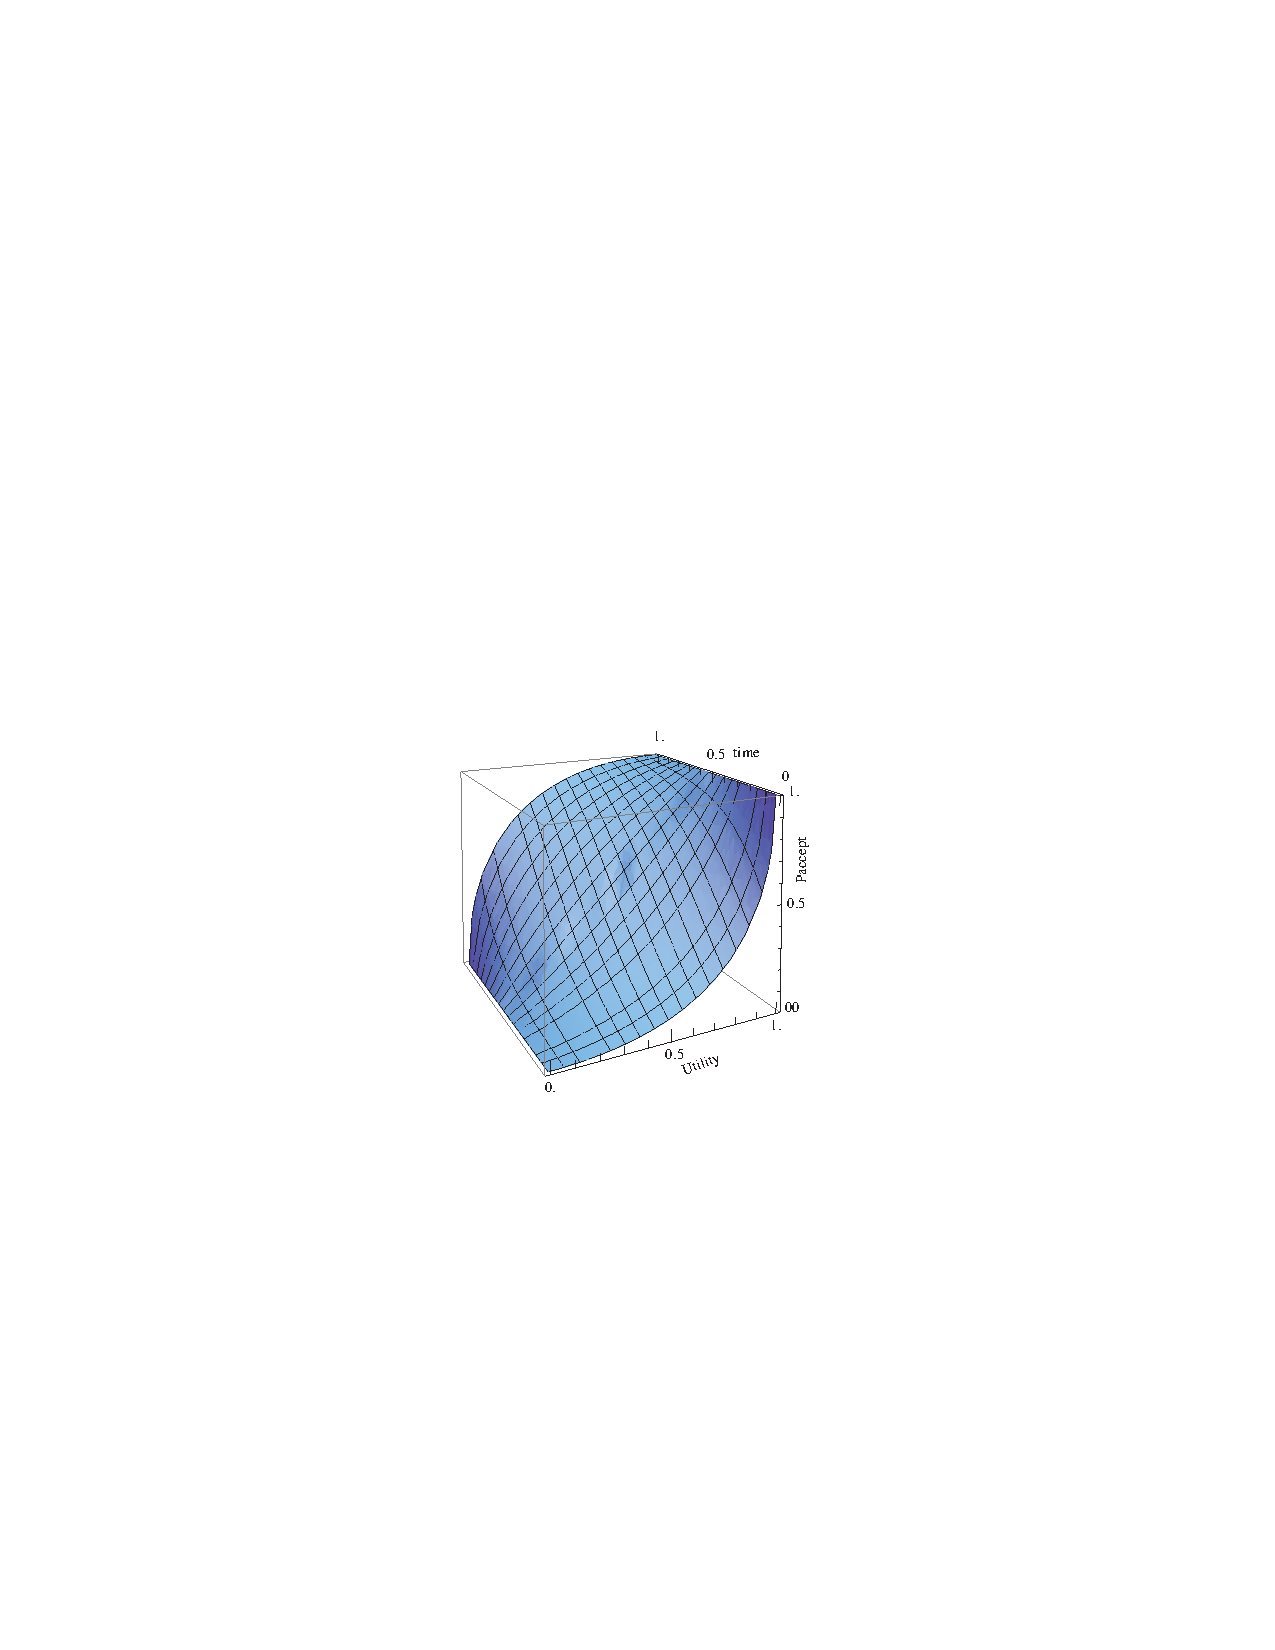
\includegraphics[width=0.3\textwidth]{media/image21.pdf}
	\caption{$P_\text{accept}$ value as function of the utility and time (as a fraction of the total available time).}\label{Fig:Paccept}
\end{figure}
%\subsection{Init}
%An important consideration for the implementation is that an agent may participate in multiple negotiation sessions with the same opponent. This enables the agent to learn from the previous sessions. For this reason, the negotiation environment calls the method \texttt{init} before starting the new session.
 
Automatic agents have to negotiate on their own, and are not allowed to communicate with a human user. Therefore, do not override the \texttt{isUIAgent()} function in automatic negotiation agents.

\subsection{Overview of Classes}
This section provides an overview of classes which might be useful when implementing an agent. For the documentation of the data structures that are presented, please refer to the Javadoc that can be found in your download of \Genius. 

\begin{itemize}

\item \textbf{BidDetails} is a structure to store a bid and its utility.
\item \textbf{BidDetailsTime} is a structure to store a bid, its utility, and the time of offering.
\item \textbf{BidHistory} is a structure to keep track of the bids presented by the agent and the opponent.
\item \textbf{BidIterator} is a class used to enumerate all possible bids. Also see \textit{SortedOutcomeSpace}.
\item \textbf{Pair} is a simple pair of two objects.
\item \textbf{Range} is a structure used to describe a continuous range.
\item \textbf{SortedOutcomeSpace} is a structure which stores all possible bids and their utilities. This class implements efficient search algorithms which can be used to efficiently search the space of possible bids for bids satisfying specific properties.
\item \textbf{UtilitySpace} is a representation of a preference profile. It is recommended to use this class when implementing a model of the opponent's preference profile.
\end{itemize}

\subsection{Compiling an Agent}
Compiling an agent can be done in two ways. First, in Eclipse you can simply find the compiled agent in the ``bin'' folder in your workspace. Alternatively, it is possible to compile the agent by placing \texttt{YourAgent.java} in the directory containing the \texttt{negotiator.jar} file, and using the command line: \texttt{javac -cp negosimulator.jar YourAgent.java}.

The next step is to load the agent in \Genius. Towards this end, first we should move the agent to the directory of \Genius. Note that the directory in which the agent should be put depends on your project. If for example you have a project with a package ``agents'' in which the agent is located, then the agent should be moved in a folder ``agents'' in the root of your \Genius~installation. An agent may consist of multiple class files. Now we can add the agent in one of the following two ways:

\begin{itemize}	
\item \textbf{Loading the agent using the GUI}. An agent can be easily added by going to the ``Agents'' tab in the ``Components Window'' (see Figure~\ref{fig:addAgent}). Next, pressing right click opens a popup with the option to add a new agent. The final step is to select the main class of your agent.

\begin{figure}[h] 
	\center
	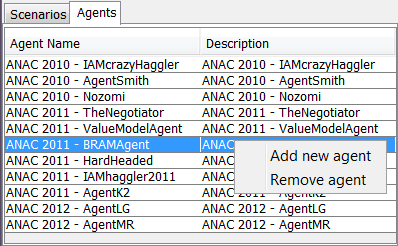
\includegraphics[width=5.5cm]{media/AddAgent.png}
	\caption{Adding an agent using the GUI.}
	\label{fig:addAgent}
\end{figure}

\item \textbf{Loading the agent using XML}. A compiled agent can also be loaded by directly adding the agent to the repository using the \textit{agentrepository.xml} file. The code below visualizes a repository with a single agent. An agent element consists of several subelements; the first element is the \textit{description} of the agent which is visualized in the GUI; the second element is the \textit{classPath} specifying were the compiled agent class is located; the third element specifies the \textit{agentName}; finally the optional element \textit{params} specifies the parameters and their values available to the agent. In this case, a parameter ``e'' with value 2 and a parameter ``time'' with value 0.95 is specified. Variables can be accessed during the negotiation by using the \textit{getStrategyParameters} method.
\end{itemize}

\begin{lstlisting}
<?xml version="1.0" encoding="UTF-8" standalone="yes"?>
<repository fileName="agentrepository.xml">
  <items>
   <agentRepItems>
     <agentRepItem description="Other agents - SimpleAgent"
			classPath="agents.SimpleAgent"
			agentName="SimpleAgent" params="e=2;time=0.95"/>
     </agentRepItems>
  </items>
<filename>agentrepository.xml</filename>
</repository>
\end{lstlisting}

\section{Creating a BOA Agent}\label{sec:boa}
Instead of implementing your negotiating agent from scratch, we recommend you create a BOA agent using the \textit{BOA framework}. The BOA negotiation agent architecture allows to reuse existing components from other BOA agents. Many of the sophisticated agent strategies that currently exist are comprised of a fixed set of modules. Generally, a distinction can be made between four different modules: one module that decides whether the opponent's bid is acceptable (\textit{acceptance strategy}); one that decides which set of bids could be proposed next (\textit{bidding strategy}); one that tries to guess the opponent's preferences (\textit{opponent model}), and finally a component which specifies how the opponent model is used to select a bid for the opponent (\textit{opponent model strategy}). The overall negotiation strategy is a result of the interaction between these components.

The advantages of separating the negotiation strategy into these four components (or equivalently, fitting an agent into the BOA framework) are threefold: first, it allows to \textit{study the performance of individual components}; second, it allows to \textit{systematically explore the space of possible negotiation strategies}; third, the reuse of existing components \textit{simplifies the creation of new negotiation strategies}.

\subsection{Components of the BOA Framework}
A negotiation agent in the BOA framework, called a \textit{BOA agent}, consists of four components:
\begin{description}
  \item[Bidding strategy] A bidding strategy is a mapping which maps a negotiation trace to a bid. The bidding strategy can interact with the opponent model by consulting with it.%, passing one or multiple bids and see how they compare within the opponent's utility space.

  \item[Opponent model] An opponent model is in the BOA framework a learning technique that constructs a model of the opponent's preference profile.% In our approach, the opponent model should be able to estimate the opponent's utility of a given bid.
  \item[Opponent model strategy] Specifies how the opponent model is used to select a bid for the opponent and the opponent model may be updated in a turn as updating the opponent model the whole negotiation may be computationally expensive.
  \item[Acceptance strategy] The acceptance strategy determines whether the opponent's bid is acceptable.
\end{description}
The components interact in the following way (the full process is visualized in Figure~\ref{fig:flowchart}). When receiving a bid, the BOA agent first  updates the \textit{bidding history}. Next, the \textit{opponent model strategy} is consulted if the \textit{opponent model} may be updated this turn. If so, the \textit{opponent model} is updated.

Given the opponent's bid, the \textit{bidding strategy} determines the counter offer by first generating a set of bids with a similar preference for the agent. The \textit{bidding strategy} uses the \textit{opponent model strategy} to select a bid from this set taking the opponent's utility into account.

Finally, the \textit{acceptance strategy} decides whether the opponent's action should be accepted. If the opponent's bid is not accepted by the acceptance strategy, then the generated bid is presented instead.

\begin{figure}[t] 
	\center
	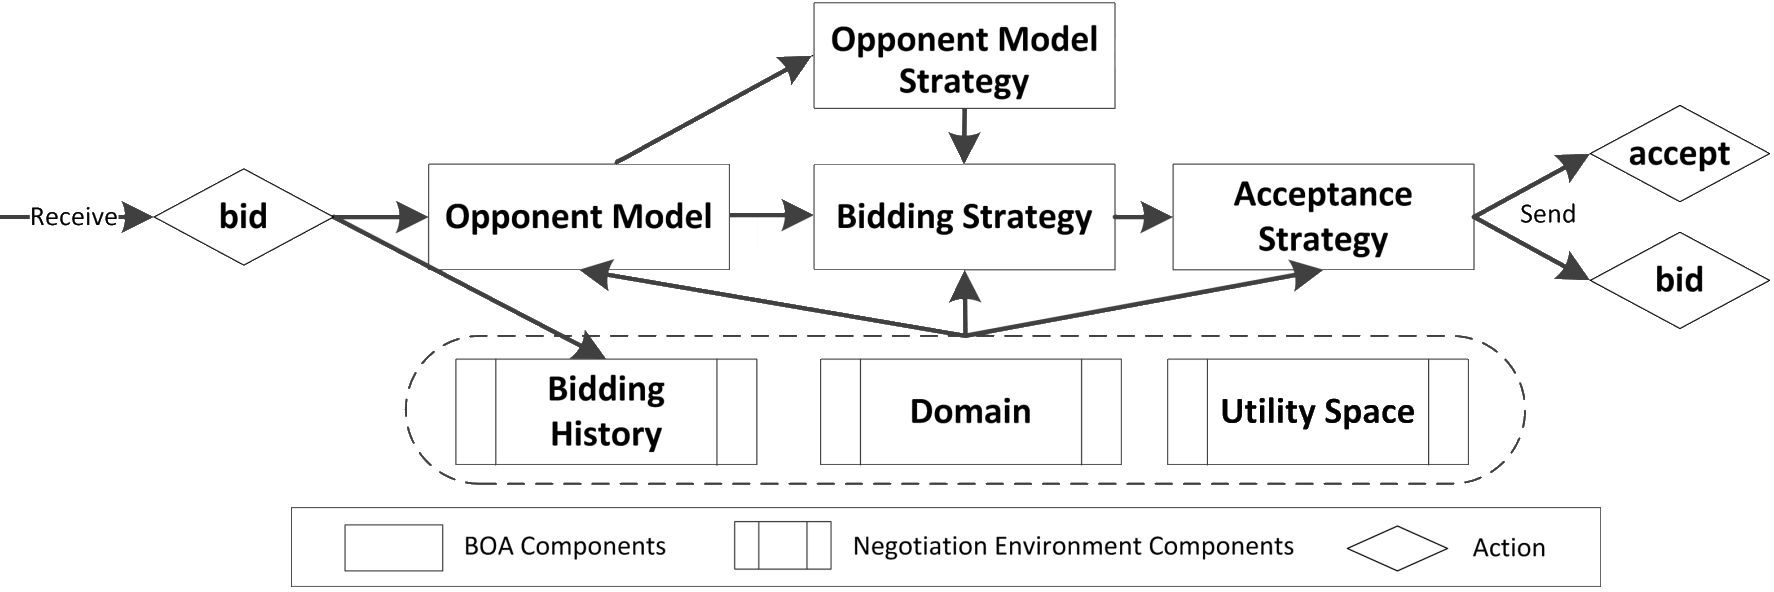
\includegraphics[width=15.0cm]{media/BOAflow.png}
	\caption{The BOA Framework Architecture.}
	\label{fig:flowchart}
\end{figure}
\pagebreak
\subsection{Using Existing Components}
In this section we create a \textit{BOA agent} by selecting its components from a list of existing components. The BOA framework GUI (see Figure~\ref{fig:decoupledGUI}) can be opened by double clicking the \textit{Values} section next to the \textit{BOA Agent side A} or \textit{BOA Agent side B} when creating a (distributed) tournament.

\begin{figure}[h!]
	\center
	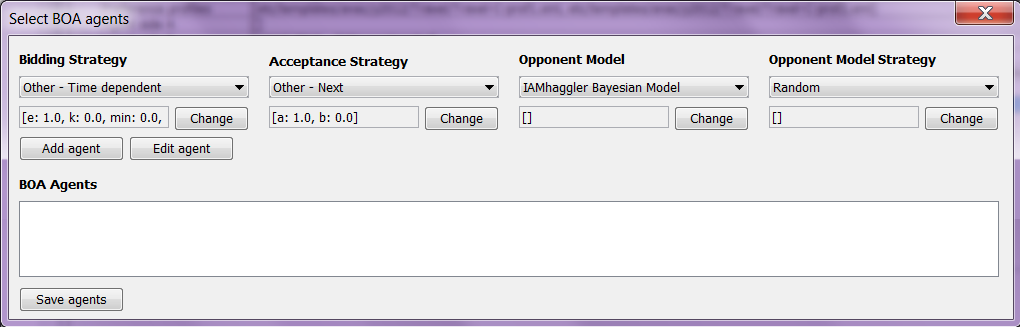
\includegraphics[width=15cm]{media/BOAgui.png}
	\caption{The BOA framework GUI.}
	\label{fig:decoupledGUI}
\end{figure}

Our goal in this section is to specify three BOA agents which are equal except for a single parameter $a$ of their acceptance strategy. First, we select the bidding strategy \textit{Other - Time Dependent} under the heading \textit{Bidding Strategy}. Note that when we select this strategy, the default parameters of the component appear in the textbox below. Next, we select the other three components shown in Figure~\ref{fig:decoupledGUI}.

The next step is to specify three variants of the acceptance strategy differing in the parameter $a$. To be more precise, we want $a$ to be 1.0, 1.1, and 1.2. To achieve this, select ``Change'' to open a window similar to Figure~\ref{fig:boaparam}. Next, fill in the fields as shown in Figure~\ref{fig:boaparam}. Finally, we select ``Add agent(s)'' to create the three agents. Note that in this example we only varied a single parameter of a single component. If we vary more parameters possibly of different components, then all possible combinations are generated.

\begin{figure}[h!] 
	\center
	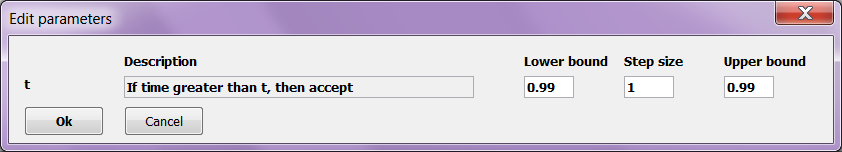
\includegraphics[width=15cm]{media/BOAparam.png}
	\caption{Adding a parameter.}
	\label{fig:boaparam}
\end{figure}

\subsection{Creating New Components}
This section discusses how create your own components. An example implementation of each component is included in the ``BOA example'' folder. The next section discusses how these components can be added to the list of available components in the BOA framework GUI.

\subsubsection{Creating a Bidding Strategy}
A bidding strategy can be easily created by extending the \textit{OfferingStrategy} class. Table~\ref{tab:BOAbs} depicts the methods which need to be overridden. The \textit{init} method of the bidding strategy is automatically called by the BOA framework with four parameters: the negotiation session, the opponent model, the opponent model strategy, and the parameters of the component. The negotiation session object keeps track of the negotiation state, which includes all offers made by both agents, the timeline, the preference profile, and the domain. The parameters object specifies the parameters as specified in the GUI. In the previous section we specified the parameter $b$ for the acceptance strategy $Other - Next$ to be 0.0. In this case the agent can retrieve the value of the parameter by calling \textit{parameters.get(``b'')}.

An approach often taken by many bidding strategies is to first generate all possible bids. This can be efficiently done by using the \textit{SortedOutcomeSpace} class. For an example on using this class see the \textit{TimeDependent\_Offering} class in the \textit{BOA example} directory.

\begin{table}[h]
\begin{tabular}{m{0.9\textwidth}}
\hline
\texttt{void init(NegotiationSession negotiationSession, OpponentModel opponentModel, 
						OMStrategy omStrategy, HashMap<String, Double> parameters)}\\
Method directly called after creating the agent which should be used to initialize the component.\\
\hline
\texttt{BidDetails determineOpeningBid()}\\
Method which determines the first bid to be offered to the component.\\
\hline
\texttt{BidDetails determineNextBid()}\\
Method which determines the bids offered to the opponent after the first bid.\\
\hline
\end{tabular}
\caption{The main methods of the bidding strategy component.}
\label{tab:BOAbs}
\end{table}


\subsubsection{Creating an Acceptance Condition}
This section discusses how to create an acceptance strategy class by extending the abstract class \textit{AcceptanceStrategy}. Table~\ref{tab:BOAas} depicts the two methods which need to specified.

\begin{table}[h]
\begin{tabular}{m{0.9\textwidth}}
\hline
\texttt{void init(NegotiationSession negotiationSession, OfferingStrategy offeringStrategy
						HashMap<String, Double> parameters)}\\
Method directly called after creating the agent which should be used to initialize the component.\\
\hline
\texttt{Actions determineAcceptability()}\\
Method which determines if the agent should accept the opponent's bid (\textit{Actions.Accept}), reject it and send a counter offer (\textit{Actions.Reject}), or leave the negotiation (\textit{Actions.Break}).\\
\hline
\end{tabular}
\caption{The main methods of the acceptance strategy component.}
\label{tab:BOAas}
\end{table}

\subsubsection{Creating an Opponent Model}
This section discusses how to create an opponent model by extending the abstract class \textit{OpponentModel}. Table~\ref{tab:BOAom} provides an overview of the main methods which need to specified. For performance reasons it is recommended to use the \textit{UtilitySpace} class.

\begin{table}[h]
\begin{tabular}{m{0.9\textwidth}}
\hline
\texttt{void init(NegotiationSession negotiationSession, HashMap<String, Double> parameters)}\\
Method directly called after creating the agent which should be used to initialize the component.\\
\hline
\texttt{double getBidEvaluation(Bid bid)}\\
Returns the estimated utility of the given bid.\\
\hline
\texttt{double updateModel(Bid bid)}\\
Updates the opponent model using the given bid.\\
\hline
\texttt{UtilitySpace getOpponentUtilitySpace()}\\
Returns the opponent's preference profile. Use the \textit{UtilitySpaceAdapter} class when not using the utilityspace class for the opponent's preference profile.\\
\hline
\end{tabular}
\caption{The main methods of the opponent model component.}
\label{tab:BOAom}
\end{table}

\subsubsection{Creating an Opponent Model Strategy}
This section discusses how to create an opponent model strategy by extending the abstract class \textit{OMStrategy}. Table~\ref{tab:BOAoms} provides an overview of the main methods which need to specified.

\begin{table}[h]
\begin{tabular}{m{0.9\textwidth}}
\hline
\texttt{void init(NegotiationSession negotiationSession, OpponentModel model, HashMap<String, Double> parameters)}\\
Method directly called after creating the agent which should be used to initialize the component.\\
\hline
\texttt{BidDetails getBid(List<BidDetails> bidsInRange);}\\
This method returns a bid to be offered from a set of given similarly preferred bids by using the opponent model.\\
\hline
\texttt{boolean canUpdateOM();}\\
Determines if the opponent model may be updated this turn.\\
\hline
\end{tabular}
\caption{The main methods of the opponent model strategy component.}
\label{tab:BOAoms}
\end{table}

\subsection{Adding a Component to the BOA Repository}
In the previous section we discussed how to create each type of BOA component. To use the components, we still need to add them to the \textit{BOA repository}. The \textit{BOA repository} is located in the main directory of \Genius ~and its structure is similar to the small repository shown below. There are four main categories corresponding to the component types. Each element in a category has to specify a description and a classpath. Optionally, one or multiple parameters may be specified.

\begin{lstlisting}
<?xml version="1.0" encoding="UTF-8" standalone="yes"?>
<repository fileName="boarepository.xml">
  <biddingstrategies>
    <biddingstrategy description="2010 - IAMcrazyHaggler"
		classPath="negotiator.boaframework.offeringstrategy.
		anac2010.IAMCrazyHaggler_Offering">
		<parameter name="b" default="0.9" description="Minimum utility"/>
    </biddingstrategy>
  </biddingstrategies>
  <acceptanceconditions>
    <acceptancecondition description="Other - False"
		classPath="negotiator.boaframework.acceptanceconditions.other.AC_False"/>
  </acceptanceconditions>
  <opponentmodels>
    <opponentmodel description="AgentX Frequency Model"
		classPath="negotiator.boaframework.opponentmodel.AgentXFrequencyModel"/>
  </opponentmodels>
  <omstrategies>
    <omstrategy description="Best bid"
		classPath="negotiator.boaframework.omstrategy.BestBid"/>
  </omstrategies>
</repository>
\end{lstlisting}
\pagebreak
\subsection{Advanced: Converting a BOA Agent to an Agent}
To convert a BOA agent to a normal agent you have to create a class that extends \textit{BOA agent} and override the \textit{agentSetup} method. Below is an example of a BOA agent wrapped as a normal agent.

\begin{lstlisting}
public class SimpleBOAagent extends BOAagent{

	@Override
	public void agentSetup() {
		OpponentModel om = new FrequencyModel(negotiationSession, 0.2, 1);
		OMStrategy oms = new NullStrategy(negotiationSession);
		OfferingStrategy offering  = new TimeDependent_Offering(negotiationSession,
								om, oms, 0.2, 0, 1, 0);
		AcceptanceStrategy ac = new AC_Next(negotiationSession, offering, 1, 0);
		setDecoupledComponents(ac, offering, om, oms);		
	}

	@Override
	public String getName() {
		return "SimpleBOAagent";
	}
}
\end{lstlisting}

\subsection{Advanced: Multi-Acceptance Criteria (MAC)}
The \textit{BOA framework} allows us to better explore a large space of negotiation strategies. MAC can be used to scale down the negotiation space, and thereby make it more computationally explorable.

As discussed in the introduction of this chapter, the acceptance condition determines solely if a bid should be accepted. This entails that it does not influence the bidding trace, except for when it is stopped. In fact, the only difference between \textit{BOA agents} where only the acceptance condition vary, is the time of agreement (assuming that the computational cost of the acceptance conditions are negligible).

Given this property, multiple acceptance criteria can be tested in parallel during the same negotiation trace. In practice, more than 50 variants of for example $\textbf{AC}_{next}$ can be tested in the same negotiation at a negligible computational cost.

To create a multi-acceptance condition component you first need to extend the class \textit{Mulit Acceptance Condition}, this gives access to the ACList which is a list of acceptance conditions to be tested in parallel. An acceptance can be added to the MAC by appending it to the AClist as sown below.

\begin{lstlisting}
public class AC_MAC extends Multi_AcceptanceCondition {
	@Override
	public void init(NegotiationSession negoSession, OfferingStrategy strat, 
			HashMap<String, Double> parameters) throws Exception {
		this.negotiationSession = negoSession;
		this.offeringStrategy = strat;
		outcomes = new ArrayList<OutcomeTuple> ();
		ACList = new ArrayList<AcceptanceStrategy>();
		for (int e = 0; e < 5; e++) {
			ACList.add(new AC_Next(negotiationSession, offeringStrategy, 1, 
												e * 0.01));
		}
	}
}

\end{lstlisting}

\section{Conclusion}
This concludes the manual of \Genius. If you experience problems or have suggestions on how to improve \Genius, please send them to \url{ai@mmi.tudelft.nl}.


%\bibliographystyle{plain}
%\bibliography{}
\end{document}